\documentclass[10pt,aspectratio=169]{beamer}

\usetheme{Madrid}
\usecolortheme{dove}
\usefonttheme{serif}
\setbeamertemplate{navigation symbols}{}
\setbeamertemplate{caption}[numbered]
\setbeamertemplate{footline}{%
  \leavevmode\hbox{%
  \begin{beamercolorbox}[wd=.38\paperwidth,ht=2.6ex,dp=1.1ex,leftskip=1em]{author in head/foot}%
    \scriptsize Q-Reliability Lab
  \end{beamercolorbox}%
  \begin{beamercolorbox}[wd=.48\paperwidth,ht=2.6ex,dp=1.1ex,center]{title in head/foot}%
    \scriptsize \insertsection
  \end{beamercolorbox}%
  \begin{beamercolorbox}[wd=.14\paperwidth,ht=2.6ex,dp=1.1ex,rightskip=1em plus 1fil]{date in head/foot}%
    \scriptsize \insertframenumber/\inserttotalframenumber
  \end{beamercolorbox}}\vskip0pt}
\setbeamertemplate{headline}{}
\setbeamersize{text margin left=8mm,text margin right=8mm}
\setlength{\tabcolsep}{4pt}
\renewcommand{\arraystretch}{1.12}

\usepackage{amsmath,amssymb,booktabs,braket,graphicx,siunitx}
\usepackage[font=small,labelfont=bf]{caption}
\graphicspath{{../paper/figures/}}
\definecolor{quantumblue}{RGB}{25,73,118}
\definecolor{quantumred}{RGB}{148,40,47}
\setbeamercolor{structure}{fg=quantumblue}
\setbeamercolor{frametitle}{fg=quantumblue}
\setbeamercolor{title}{fg=quantumblue}
\newcommand{\sourcefoot}[1]{\vfill\tiny\color{gray}Source: #1}

\title[Q-Reliability Lab]{Q-Reliability Lab}
\subtitle{Computational-basis success can remain perfect while phase-flip noise destroys the target Bell-state relation}
\author{Zhen-Jun Liu}
\institute{Independent research project}
\date{30 October 2026}

\begin{document}

\begin{frame}
  \titlepage
  \vfill
  \begin{center}
  \small Classical density-matrix simulation with deterministic finite-shot sampling; no quantum-hardware data.
  \end{center}
\end{frame}

\begin{frame}{Outline}
\begin{columns}[T]
\column{.49\textwidth}
\begin{enumerate}
  \item Motivation and precise research question
  \item Phase-flip model and analytic predictions
  \item Basis-sensitive success metrics
  \item Exact density-matrix sweep
\end{enumerate}
\column{.49\textwidth}
\begin{enumerate}
  \setcounter{enumi}{4}
  \item Finite-shot experiment and uncertainty
  \item Channel--metric sensitivity comparison
  \item Reproducibility, limits, and implications
  \item Conclusions and future work
\end{enumerate}
\end{columns}
\vspace{3mm}
\begin{block}{Seminar claim}
For a Bell-state benchmark, a success definition based only on accepted computational-basis populations cannot certify the relative phase of the state.
\end{block}
\sourcefoot{Project source, analytic record, and committed experiment artifacts.}
\end{frame}

\section{Question and model}
\begin{frame}[plain]
\vfill\centering
{\color{quantumblue}\LARGE Question and model}\par\vspace{3mm}
\large A Bell-state benchmark under a first-qubit phase-flip channel
\vfill
\end{frame}

\begin{frame}[t]{Motivation: accepted outcomes can hide state damage}
\begin{columns}[T]
\column{.50\textwidth}
\begin{itemize}
  \item Bell-state preparation targets $\ket{\Phi^+}=(\ket{00}+\ket{11})/\sqrt{2}$.
  \item A computational-basis task can accept both $00$ and $11$, reporting $S_Z=P(00)+P(11)$.
  \item $\ket{\Phi^+}$ and $\ket{\Phi^-}=(\ket{00}-\ket{11})/\sqrt{2}$ have the same accepted populations.
  \item Their relative phase differs, so agreement with the intended target differs.
\end{itemize}
\column{.50\textwidth}
\begin{block}{Concrete failure mode}
At $p=1$, the output becomes $\ket{\Phi^-}$:\\[1mm]
\centering $S_Z=1$ \qquad $F_{\Phi^+}=0$.
\end{block}
\begin{alertblock}{Reliability question}
Does a perfect task success score actually establish preparation of the desired Bell state?
\end{alertblock}
\end{columns}
\sourcefoot{Analytic setup in \texttt{paper/main.tex}, Introduction and Methodology.}
\end{frame}

\begin{frame}[t]{Bell state and phase-flip channel}
\begin{columns}[T]
\column{.54\textwidth}
\begin{align*}
\ket{\Phi^+}&=\frac{\ket{00}+\ket{11}}{\sqrt2},\\
\rho_+&=\frac12\begin{pmatrix}1&0&0&1\\0&0&0&0\\0&0&0&0\\1&0&0&1\end{pmatrix}.\\[-1mm]
E_0&=\sqrt{1-p}\,I_4,\qquad E_1=\sqrt p\,(Z\otimes I).
\end{align*}
\begin{itemize}
  \item Ordered basis: $(\ket{00},\ket{01},\ket{10},\ket{11})$.
  \item Noise acts only after the ideal Bell circuit.
  \item $p\in[0,1]$ denotes the channel probability.
\end{itemize}
\column{.46\textwidth}
\begin{block}{Kraus completeness}
\[
\sum_k E_k^\dagger E_k=(1-p)I_4+p(Z\otimes I)^2=I_4.
\]
\end{block}
\begin{block}{Physical interpretation}
$(Z\otimes I)\ket{\Phi^+}=\ket{\Phi^-}$, so the channel mixes two orthogonal Bell states.
\end{block}
\end{columns}
\sourcefoot{Kraus construction and completeness: \texttt{src/phase\_error\_blind\_spot.py}.}
\end{frame}

\begin{frame}[t]{Central question and hypothesis}
\begin{block}{Question}
For the stated phase-flip model, which measured quantities remain informative as $p$ changes from zero to one?
\end{block}
\begin{columns}[T]
\column{.50\textwidth}
\textbf{Hypothesis}\par
\vspace{1mm}
The computational-basis correlated-success metric is structurally insensitive to the phase flip, while fidelity, signed coherence, and an X-basis correlation expose the change.
\vspace{3mm}
\begin{itemize}
  \item Exact sweep: 101 values, $p=0.00,0.01,\ldots,1.00$.
  \item Finite-shot sweep: five $p$ values, three shot budgets, two bases, 100 repetitions.
\end{itemize}
\column{.50\textwidth}
\begin{block}{Claim boundary}
The study reproduces a known measurement-basis limitation as a transparent benchmark. It does not introduce a new noise model or estimate a hardware error rate.
\end{block}
\begin{block}{Falsifiable contrast}
If $S_Z$ falls with $p$ under this model, the analytic derivation or implementation is incorrect.
\end{block}
\end{columns}
\sourcefoot{Scope statement: \texttt{docs/self\_audit.md}; model: \texttt{paper/main.tex}.}
\end{frame}

\begin{frame}[t]{Exact analytic baseline}
\begin{columns}[T]
\column{.57\textwidth}
\[
\rho(p)=\frac12\begin{pmatrix}
1&0&0&1-2p\\0&0&0&0\\0&0&0&0\\1-2p&0&0&1
\end{pmatrix}.
\]
\begin{align*}
S_Z(p)&=1, & F_{\Phi^+}(p)&=1-p,\\
\mathrm{Re}\,\rho_{00,11}(p)&=\frac{1-2p}{2}, &
|\rho_{00,11}(p)|&=\frac{|1-2p|}{2}.
\end{align*}
\column{.43\textwidth}
\begin{tabular}{@{}cccc@{}}
\toprule
$p$ & $S_Z$ & $F$ & $\mathrm{Re}\,\rho_{00,11}$\\
\midrule
0.00 & 1.00 & 1.00 & 0.50\\
0.50 & 1.00 & 0.50 & 0.00\\
1.00 & 1.00 & 0.00 & -0.50\\
\bottomrule
\end{tabular}
\vspace{3mm}
\begin{block}{Endpoint interpretation}
$p=0.5$ removes coherence. $p=1$ reverses its sign and produces a state orthogonal to the target.
\end{block}
\end{columns}
\sourcefoot{Values from \texttt{experiments/phase\_error\_sweep.csv}; formulas in \texttt{paper/main.tex}.}
\end{frame}

\section{Metrics and exact sweep}
\begin{frame}[plain]
\vfill\centering
{\color{quantumblue}\LARGE Metrics and exact sweep}\par\vspace{3mm}
\large Success definitions determine which errors a benchmark can observe
\vfill
\end{frame}

\begin{frame}[t]{Z-basis and X-basis correlated success}
\begin{columns}[T]
\column{.55\textwidth}
\begin{align*}
S_Z(\rho)&=\rho_{00,00}+\rho_{11,11},\\
\Pi_X&=\ket{++}\!\bra{++}+\ket{--}\!\bra{--},\\
S_X(\rho)&=\mathrm{Tr}(\Pi_X\rho)\\
&=\tfrac12(\rho_{00,00}+\rho_{11,11}+\rho_{00,11}+\rho_{11,00}).
\end{align*}
\begin{itemize}
  \item Code evaluates $S_X$ from the projector, rather than hardcoding $1-p$.
  \item $S_Z$ uses only populations; $S_X$ also uses off-diagonal coherence.
\end{itemize}
\column{.45\textwidth}
\begin{tabular}{@{}p{.28\textwidth}p{.52\textwidth}@{}}
\toprule
Metric & Information tested\\
\midrule
$S_Z$ & Computational-basis correlated populations\\
$S_X$ & Relative phase through X-basis correlation\\
Fidelity & Agreement with the specified $\ket{\Phi^+}$ target\\
Signed coherence & Direction and size of $\rho_{00,11}$\\
\bottomrule
\end{tabular}
\end{columns}
\sourcefoot{Projector metric: \texttt{src/phase\_error\_blind\_spot.py}; tests: \texttt{tests/test\_x\_basis\_diagnostic.py}.}
\end{frame}

\begin{frame}[t]{Structural blindness of computational-basis success}
\begin{columns}[T]
\column{.58\textwidth}
\begin{align*}
\rho_{00,00}(p)&=\tfrac12,\\
\rho_{11,11}(p)&=\tfrac12,\\
S_Z(p)&=\rho_{00,00}(p)+\rho_{11,11}(p)=1.
\end{align*}
\begin{itemize}
  \item The diagonal populations remain fixed under a $Z$ operation on the first qubit.
  \item Only the cross terms acquire the factor $1-2p$.
  \item Therefore additional Z-basis samples cannot reveal $p$ in this model.
\end{itemize}
\column{.42\textwidth}
\begin{block}{Structural, not numerical}
The constancy follows from the channel and measurement projector. It does not result from a coarse probability grid, floating-point rounding, or insufficient shot count.
\end{block}
\begin{alertblock}{Benchmark implication}
A task score may measure a valid but incomplete property of the output state.
\end{alertblock}
\end{columns}
\sourcefoot{Index-level derivation: \texttt{paper/main.tex}, Eq. $\rho(p)$ and metric definitions.}
\end{frame}

\begin{frame}[t]{Exact density-matrix sweep}
\begin{columns}[T]
\column{.61\textwidth}
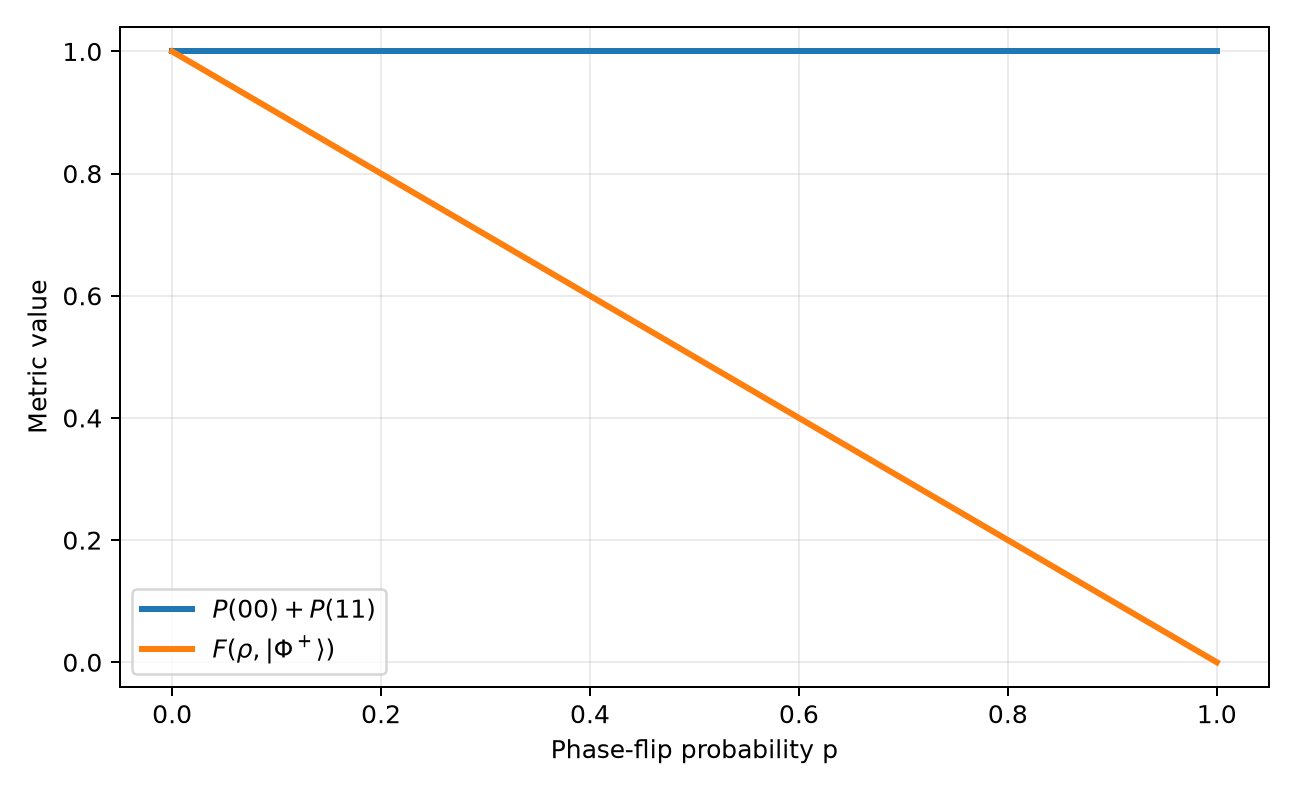
\includegraphics[width=\linewidth,height=.67\textheight,keepaspectratio]{success_vs_fidelity.png}
\column{.39\textwidth}
\begin{itemize}
  \item The exact simulator applies the Kraus map to $\rho_+$ at 101 values of $p$.
  \item $S_Z$ remains equal to one across the entire sweep.
  \item $S_X$ and fidelity both decrease linearly as $1-p$.
  \item The visual agreement reflects shared analytic predictions, checked by parameterized tests.
\end{itemize}
\begin{block}{Conclusion}
The selected Z-basis task accepts an output whose target-state fidelity falls continuously from one to zero.
\end{block}
\end{columns}
\sourcefoot{Generated by \texttt{python -m src.phase\_error\_blind\_spot}; figure: \texttt{paper/figures/success\_vs\_fidelity.png}.}
\end{frame}

\begin{frame}[t]{Signed coherence distinguishes loss from phase reversal}
\begin{columns}[T]
\column{.61\textwidth}
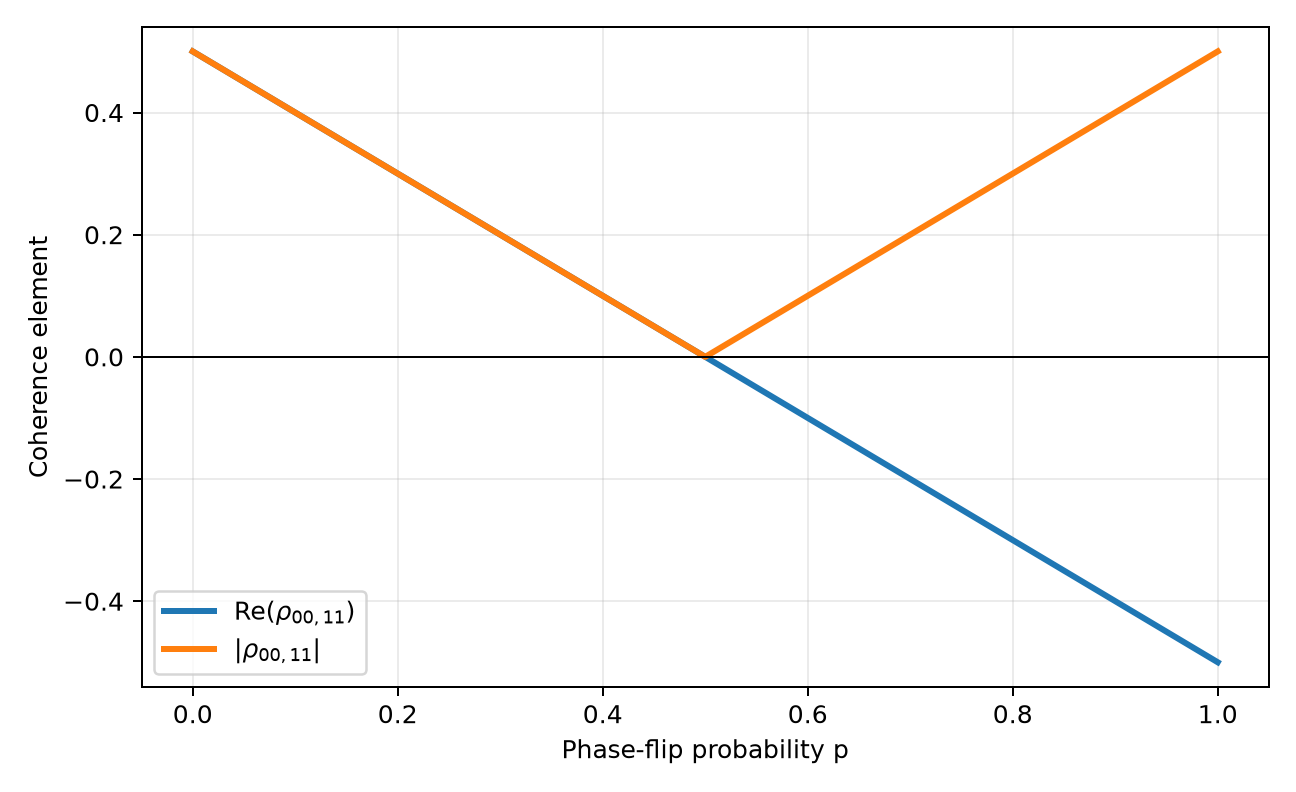
\includegraphics[width=\linewidth,height=.67\textheight,keepaspectratio]{coherence_real_vs_magnitude.png}
\column{.39\textwidth}
\begin{itemize}
  \item $|\rho_{00,11}|$ decreases to zero at $p=0.5$ and returns to $0.5$ at $p=1$.
  \item The magnitude alone cannot distinguish $\ket{\Phi^+}$ from $\ket{\Phi^-}$.
  \item $\mathrm{Re}\,\rho_{00,11}$ changes sign and records the phase reversal.
\end{itemize}
\begin{block}{Interpretation}
At $p=1$, coherence survives but has the wrong sign for the target state.
\end{block}
\end{columns}
\sourcefoot{Generated by \texttt{python -m src.phase\_error\_blind\_spot}; data: \texttt{experiments/phase\_error\_sweep.csv}.}
\end{frame}

\section{Finite-shot evidence}
\begin{frame}[plain]
\vfill\centering
{\color{quantumblue}\LARGE Finite-shot evidence}\par\vspace{3mm}
\large Sampling uncertainty changes precision, not metric sensitivity
\vfill
\end{frame}

\begin{frame}[t]{Finite-shot experiment design}
\begin{columns}[T]
\column{.52\textwidth}
\begin{tabular}{@{}ll@{}}
\toprule
Design field & Committed specification\\
\midrule
$p$ values & $0,0.25,0.50,0.75,1.00$\\
Shot budgets & $100,1{,}000,10{,}000$\\
Measurement bases & $Z$ and $X$\\
Repetitions & 100 per condition\\
Root seed & 20261030\\
CSV rows & 3,000\\
Interval & two-sided 95\% Wilson\\
\bottomrule
\end{tabular}
\column{.48\textwidth}
\begin{align*}
K_Z&=N,\\
K_X&\sim\mathrm{Binomial}(N,1-p),\\
\widehat S_B&=K_B/N.
\end{align*}
\begin{itemize}
  \item Each row records its child seed, success count, estimate, analytic value, and interval endpoints.
  \item These observations are simulated binomial samples, not hardware measurements.
\end{itemize}
\end{columns}
\sourcefoot{Design and schema: \texttt{src/finite\_shot\_phase\_error.py}; data: \texttt{experiments/finite\_shot\_sweep.csv}.}
\end{frame}

\begin{frame}[t]{Finite-shot results at $p=0.50$}
\begin{columns}[T]
\column{.61\textwidth}
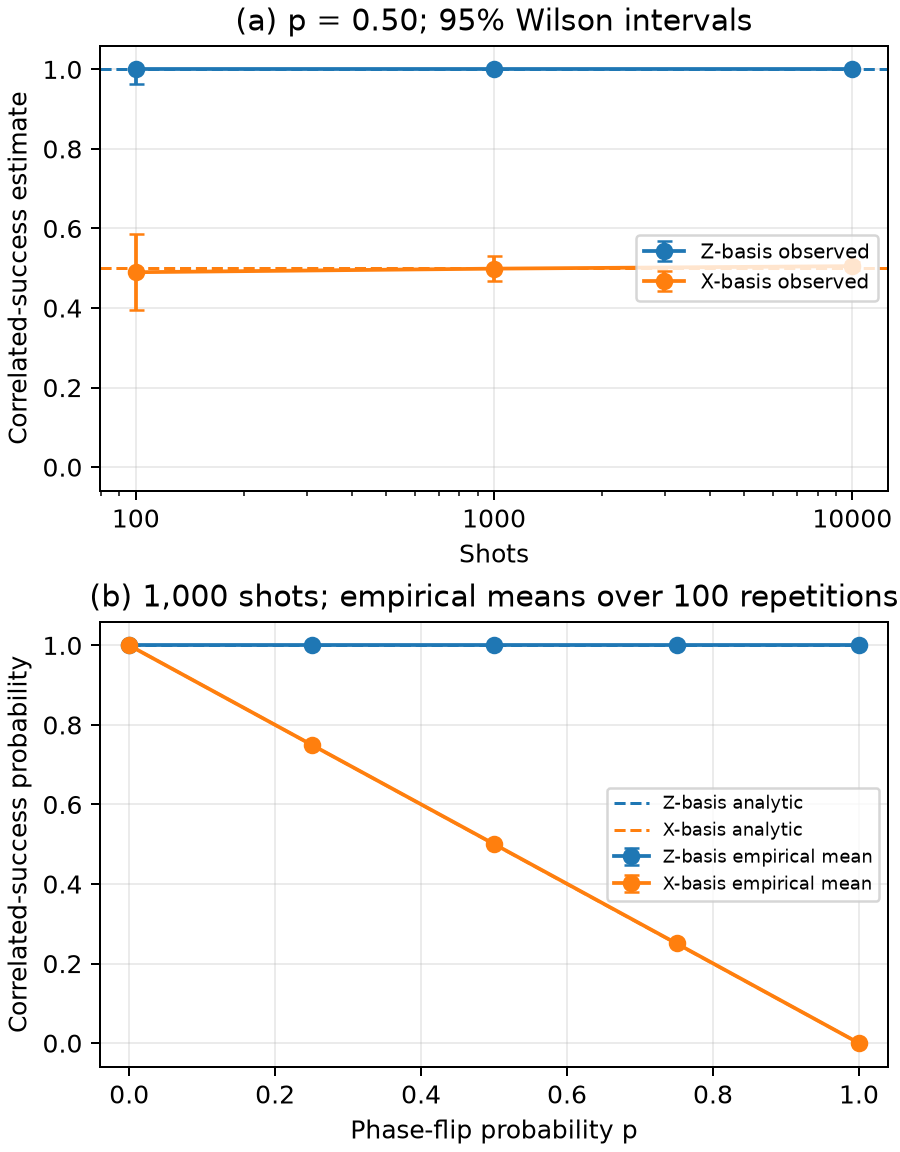
\includegraphics[width=\linewidth,height=.67\textheight,keepaspectratio]{finite_shot_detectability.png}
\column{.39\textwidth}
\begin{itemize}
  \item Every Z-basis observation reports correlated success one, for every shot budget.
  \item X-basis estimates remain close to the analytic value $S_X=0.5$.
  \item The X-basis interval narrows as $N$ increases.
  \item More samples improve an informative estimator; they do not repair an uninformative measurement basis.
\end{itemize}
\begin{block}{Conclusion}
Finite sampling introduces uncertainty around $S_X$ but leaves the Z-basis blind spot unchanged.
\end{block}
\end{columns}
\sourcefoot{Generated by \texttt{python -m src.finite\_shot\_figures}; figure data from \texttt{experiments/finite\_shot\_sweep.csv}.}
\end{frame}

\begin{frame}[t]{Wilson intervals quantify sampling precision}
\begin{columns}[T]
\column{.58\textwidth}
\begin{tabular}{@{}rrrr@{}}
\toprule
$N$ & $\widehat S_X$ & 95\% Wilson lower & upper\\
\midrule
100 & 0.4900 & 0.3942 & 0.5865\\
1,000 & 0.4990 & 0.4681 & 0.5299\\
10,000 & 0.5053 & 0.4955 & 0.5151\\
\bottomrule
\end{tabular}
\vspace{2mm}
\small All rows use $p=0.50$, basis $X$, repetition 0. The analytic success probability equals 0.5000.
\column{.42\textwidth}
\begin{itemize}
  \item Wilson intervals remain bounded at all-success and zero-success endpoints.
  \item Their width reflects finite sample size, not uncertainty about the model parameters.
  \item A Wilson interval is a frequentist confidence interval, not a posterior probability.
\end{itemize}
\end{columns}
\sourcefoot{Exact displayed values from \texttt{experiments/finite\_shot\_sweep.csv}; interval implementation in \texttt{src/finite\_shot\_phase\_error.py}.}
\end{frame}

\section{Comparative benchmark}
\begin{frame}[plain]
\vfill\centering
{\color{quantumblue}\LARGE Comparative benchmark}\par\vspace{3mm}
\large A metric can be blind to one Pauli error while detecting another
\vfill
\end{frame}

\begin{frame}[t]{Noise-channel and metric sensitivity matrix}
\begin{columns}[T]
\column{.60\textwidth}
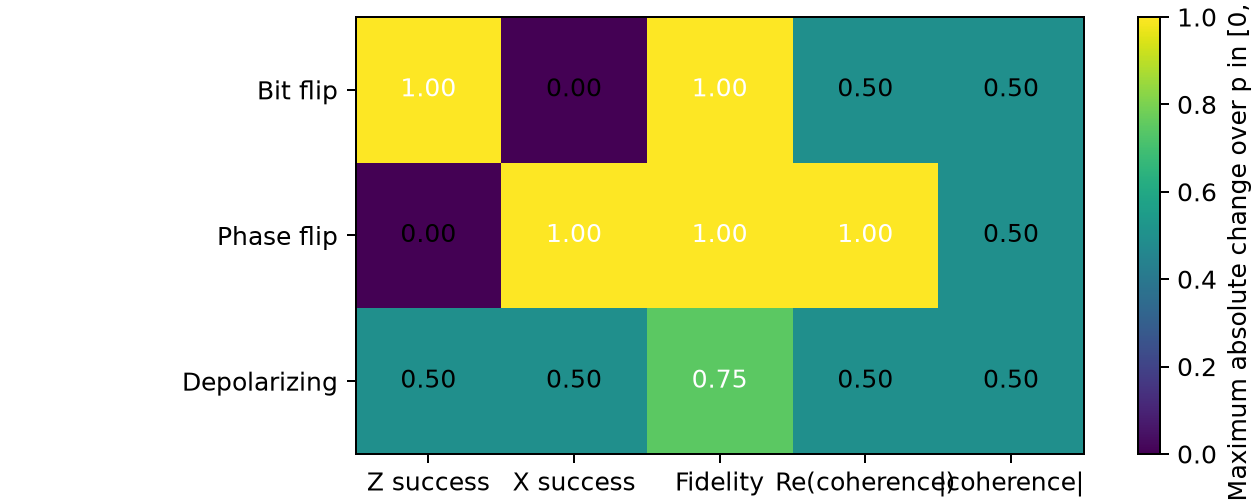
\includegraphics[width=\linewidth,height=.67\textheight,keepaspectratio]{channel_metric_sensitivity_matrix.png}
\column{.40\textwidth}
\begin{itemize}
  \item Cells report the maximum absolute metric change over $p\in[0,1]$.
  \item $S_Z$ is structurally blind to phase flips.
  \item $S_X$ is structurally blind to bit flips.
  \item Every listed metric changes under the specified depolarizing channel.
\end{itemize}
\begin{block}{Conclusion}
No single listed metric detects every modeled Pauli noise type; benchmark design must match the error mechanism.
\end{block}
\end{columns}
\sourcefoot{Generated by \texttt{python -m src.channel\_metric\_matrix}; data: \texttt{experiments/channel\_metric\_matrix.csv}.}
\end{frame}

\begin{frame}[t]{Channel comparison at the sweep endpoints}
\begin{columns}[T]
\column{.60\textwidth}
\scriptsize
\begin{tabular}{@{}lrrrrr@{}}
\toprule
Channel at $p=1$ & $S_Z$ & $S_X$ & $F$ & $\mathrm{Re}\,\rho$ & $|\rho|$\\
\midrule
Bit flip & 0.00 & 1.00 & 0.00 & 0.00 & 0.00\\
Phase flip & 1.00 & 0.00 & 0.00 & -0.50 & 0.50\\
Depolarizing & 0.50 & 0.50 & 0.25 & 0.00 & 0.00\\
\bottomrule
\end{tabular}
\vspace{2mm}
\small $\rho$ denotes the target-basis coherence element $\rho_{00,11}$.
\column{.40\textwidth}
\begin{itemize}
  \item The bit-flip and phase-flip cases exchange which basis metric remains constant.
  \item Depolarizing noise uses weights $1-3p/4,p/4,p/4,p/4$.
  \item Its target-fidelity endpoint equals $1/4$, consistent with the maximally mixed state.
\end{itemize}
\end{columns}
\sourcefoot{Values from \texttt{experiments/channel\_metric\_matrix.csv}; channel formulas in \texttt{src/channel\_metric\_matrix.py}.}
\end{frame}

\section{Reproducibility and interpretation}
\begin{frame}[plain]
\vfill\centering
{\color{quantumblue}\LARGE Reproducibility and interpretation}\par\vspace{3mm}
\large Evidence, validation boundary, and claims supported by the model
\vfill
\end{frame}

\begin{frame}[t]{Reproducibility and engineering evidence}
\begin{columns}[T]
\column{.55\textwidth}
\begin{tabular}{@{}p{.42\textwidth}p{.48\textwidth}@{}}
\toprule
Evidence & Project mechanism\\
\midrule
Exact analytics & Parameterized regression tests at five fixed $p$ values\\
Physical channel checks & Trace, Hermiticity, PSD, Kraus completeness, invalid-input tests\\
Data regeneration & Deterministic CSV sweeps and committed generated table\\
Finite-shot repeatability & Fixed root seed and stored child seed per row\\
Automation & GitHub Actions runs tests, regeneration checks, paper build, Ruff, and CodeQL\\
\bottomrule
\end{tabular}
\column{.45\textwidth}
\begin{itemize}
  \item Dependencies for CI are pinned in \texttt{requirements-ci.txt}.
  \item The CI check rejects uncommitted changes to deterministic data artifacts.
  \item The visual lab implements the same phase-flip metrics and is tested against the Python model.
\end{itemize}
\begin{block}{Reproducibility boundary}
These checks validate the stated simulation and artifacts; they do not validate quantum hardware behavior.
\end{block}
\end{columns}
\sourcefoot{Workflows: \texttt{.github/workflows}; tests: \texttt{tests/}; build notes: \texttt{docs/reproducibility.md}.}
\end{frame}

\begin{frame}[t]{Threats to validity and scope limitations}
\begin{columns}[T]
\column{.50\textwidth}
\begin{block}{Model limitations}
\begin{itemize}
  \item Classical density-matrix and binomial simulation only.
  \item One target state, one post-circuit noise location, and three Pauli channels.
  \item Ideal preparation and measurement in the exact model.
\end{itemize}
\end{block}
\begin{block}{Omitted hardware effects}
SPAM error, readout error, crosstalk, calibration drift, coherent control error, and device-specific CNOT noise.
\end{block}
\column{.50\textwidth}
\begin{block}{What the study establishes}
Within the declared channel and measurement model, the selected Z-basis success metric cannot identify phase-flip strength.
\end{block}
\begin{alertblock}{What it does not establish}
The study does not measure an IBM or other device error rate, demonstrate a fault-tolerant protocol, or provide a complete process characterization.
\end{alertblock}
\end{columns}
\sourcefoot{Detailed audit and claim boundaries: \texttt{docs/self\_audit.md} and \texttt{paper/main.tex}, Discussion.}
\end{frame}

\begin{frame}[t]{Discussion: implications for benchmark design}
\begin{columns}[T]
\column{.52\textwidth}
\begin{itemize}
  \item A metric can remain numerically stable because its measurement projector excludes the affected degree of freedom.
  \item More shots reduce uncertainty only for variation that the measurement can observe.
  \item Fidelity detects mismatch with a chosen target but does not fully characterize a general quantum process.
  \item Signed coherence adds directional phase information that coherence magnitude discards.
\end{itemize}
\column{.48\textwidth}
\begin{block}{Practical reading of a benchmark score}
Before interpreting a high score as reliable state preparation, specify: the target state, accepted outcomes, measurement basis, noise model, and uncertainty model.
\end{block}
\begin{block}{Design implication}
Use complementary observables when the task specification depends on both population and phase information.
\end{block}
\end{columns}
\sourcefoot{Interpretation grounded in the exact and finite-shot results shown in this deck.}
\end{frame}

\begin{frame}[t]{Conclusion}
\begin{columns}[T]
\column{.58\textwidth}
\begin{enumerate}
  \item The first-qubit phase-flip channel preserves $P(00)+P(11)$ for the Bell-state benchmark, so $S_Z(p)=1$ across the full sweep.
  \item The target fidelity and X-basis correlated success both equal $1-p$; they expose degradation missed by the computational-basis score.
  \item At $p=1$, the output is the coherent but target-orthogonal state $\ket{\Phi^-}$, yielding $S_Z=1$ and $F_{\Phi^+}=0$.
  \item Deterministic data, finite-shot intervals, tests, CI, and an interactive visual lab make the benchmark inspectable and reproducible.
\end{enumerate}
\column{.42\textwidth}
\begin{block}{Honest contribution}
A reproducible quantitative demonstration of a known metric blind spot, framed as a compact reliability benchmark rather than a novel physical discovery.
\end{block}
\end{columns}
\sourcefoot{All conclusions are limited to the declared classical simulation model.}
\end{frame}

\begin{frame}[t]{Future work}
\begin{columns}[T]
\column{.50\textwidth}
\begin{itemize}
  \item Extend the state family beyond $\ket{\Phi^+}$ and vary the noise location within an explicit circuit.
  \item Compare coherent over-rotation, amplitude damping, readout error, and correlated multi-qubit noise.
  \item Add tomography-inspired or randomized-benchmarking-style observables where their assumptions are explicit.
\end{itemize}
\column{.50\textwidth}
\begin{itemize}
  \item Run a separately calibrated hardware experiment with documented device, backend date, transpilation, and shot protocol.
  \item Report hardware uncertainty separately from simulation uncertainty.
  \item Evaluate whether metric blind spots persist under realistic task-level acceptance rules.
\end{itemize}
\end{columns}
\begin{block}{Next empirical step}
Hardware data would require a new experiment design; the present simulation supplies analytic controls and regression baselines for that extension.
\end{block}
\sourcefoot{Proposed extensions, not results of the current study.}
\end{frame}

\section{References}
\begin{frame}[t]{References}
\small
\begin{thebibliography}{9}
\bibitem{nielsen} M. A. Nielsen and I. L. Chuang. \emph{Quantum Computation and Quantum Information}. Cambridge University Press, 10th Anniversary Edition, 2010. doi:10.1017/CBO9780511976667.
\vspace{2mm}
\bibitem{preskill} J. Preskill. Quantum Computing in the NISQ Era and Beyond. \emph{Quantum}, 2:79, 2018. doi:10.22331/q-2018-08-06-79.
\vspace{2mm}
\bibitem{wood} C. J. Wood, J. D. Biamonte, and D. G. Cory. Tensor Networks and Graphical Calculus for Open Quantum Systems. \emph{Quantum Information and Computation}, 15(9--10):759--811, 2015.
\vspace{2mm}
\bibitem{repo} Z.-J. Liu. \emph{Q-Reliability Lab}. Version 0.1.0, 2026. Repository: \texttt{github.com/Raina-ya/q-reliability-lab}.
\end{thebibliography}
\sourcefoot{Bibliographic entries match \texttt{paper/references.bib} and \texttt{CITATION.cff}.}
\end{frame}

\appendix
\section{Backup}
\begin{frame}[t]{Backup: output-state derivation}
\begin{align*}
\mathcal E_p(\rho_+)&=(1-p)\rho_+ + p(Z\otimes I)\rho_+(Z\otimes I)\\
&=(1-p)\ket{\Phi^+}\!\bra{\Phi^+}+p\ket{\Phi^-}\!\bra{\Phi^-}.
\end{align*}
\begin{columns}[T]
\column{.56\textwidth}
\[
\rho(p)=\frac12\begin{pmatrix}
1&0&0&1-2p\\0&0&0&0\\0&0&0&0\\1-2p&0&0&1
\end{pmatrix}.
\]
\column{.44\textwidth}
\begin{itemize}
  \item Diagonal entries remain $1/2$.
  \item The coherence crosses zero at $p=1/2$.
  \item The endpoint at $p=1$ has negative coherence, not zero coherence.
\end{itemize}
\end{columns}
\sourcefoot{Full derivation: \texttt{notes/2026-10-29-analytic-phase-flip-record.md} and \texttt{paper/main.tex}.}
\end{frame}

\begin{frame}[t]{Backup: representative exact sweep values}
\centering
\small
\begin{tabular}{@{}rrrrr@{}}
\toprule
$p$ & $S_Z$ & $S_X$ & $F$ & $\mathrm{Re}\,\rho_{00,11}$\\
\midrule
0.00 & 1.00 & 1.00 & 1.00 & 0.50\\
0.25 & 1.00 & 0.75 & 0.75 & 0.25\\
0.50 & 1.00 & 0.50 & 0.50 & 0.00\\
0.75 & 1.00 & 0.25 & 0.25 & -0.25\\
1.00 & 1.00 & 0.00 & 0.00 & -0.50\\
\bottomrule
\end{tabular}
\vspace{5mm}
\begin{block}{Cross-check}
The table equals the committed CSV values and the analytic relations used in the regression tests.
\end{block}
\sourcefoot{\texttt{experiments/phase\_error\_sweep.csv} and \texttt{paper/generated/phase\_error\_results\_table.tex}.}
\end{frame}

\begin{frame}[t]{Backup: deterministic regeneration commands}
\small
\begin{block}{Exact sweep, figures, and paper table}
\texttt{python -m src.phase\_error\_blind\_spot --output experiments/phase\_error\_sweep.csv --figures paper/figures --table paper/generated/phase\_error\_results\_table.tex}
\end{block}
\begin{block}{Finite-shot data and figure}
\texttt{python -m src.finite\_shot\_phase\_error --output experiments/finite\_shot\_sweep.csv --root-seed 20261030}\\[1mm]
\texttt{python -m src.finite\_shot\_figures --input experiments/finite\_shot\_sweep.csv --output paper/figures/finite\_shot\_detectability.png}
\end{block}
\begin{block}{Channel matrix}
\texttt{python -m src.channel\_metric\_matrix --output experiments/channel\_metric\_matrix.csv --figure paper/figures/channel\_metric\_sensitivity\_matrix.png}
\end{block}
\sourcefoot{CI verifies the deterministic CSV and generated table artifacts.}
\end{frame}

\end{document}
